\documentclass{article}

\usepackage[utf8]{inputenc}
\usepackage{graphicx}
\usepackage{amsmath}
\usepackage[letterpaper, portrait, margin=1in]{geometry}
\usepackage{booktabs}

\title{Biomaterials HW 7}
\author{Nikhil Menon}
\date{October 29th, 2016}

\begin{document}

\maketitle
1. From the given parameters, we can calculate the total volume of the cell to be $9.33*10^{-23} cm^3$. Then, since there are 4 $CH_2$ groups, the total mass is 

$$\frac{4*14 (g/mol)}{6.022*10^{23} atoms/mol}=9.29*10^{-23} g$$
Therefore, the density of crystalline polyethylene is $0.996 g/cm^3$
If the fraction of the material that is crystal is $f$,
$$0.996f+0.866(1-f)=0.983 g/cm^3, f=0.89$$

2a. We know that
$$T_g=T_{\infty}-\frac{K}{M}$$
After performing a linear fit with the given $T_G$ against the inverse of the molecular weight using data,
$$T_{\infty}=379 K, K=2.1*10^5 K g mol^-{1}$$
\begin{figure}[h]
\centering
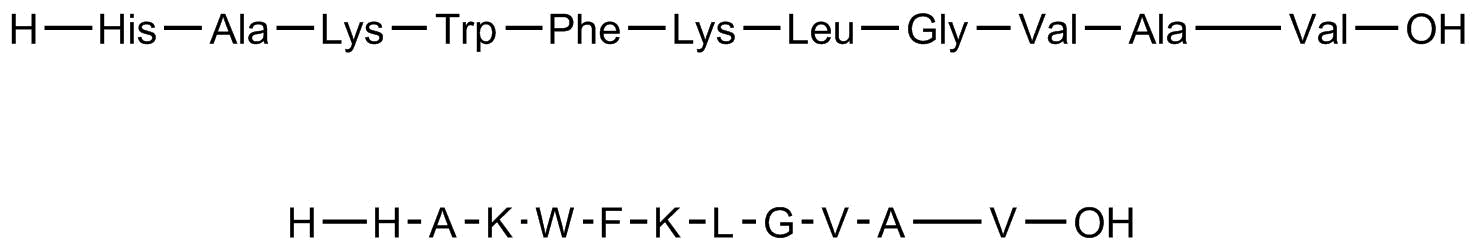
\includegraphics[scale=0.9]{P2.png}
\end{figure}

2b. For a polydisperse polymer, 
$$T_g=w_1T_{g,1}+w_2T_{g,2}+w_3T_{g,3}+w_4T_{g,4}=377 K$$

3. The $T_g$ should be about 246 K. The plotted data with the equation of best fit is shown below. The data is approximately quadratic, and this modal is a good fit as seen in the high $R^2$ value.
\begin{figure}[h]
\centering
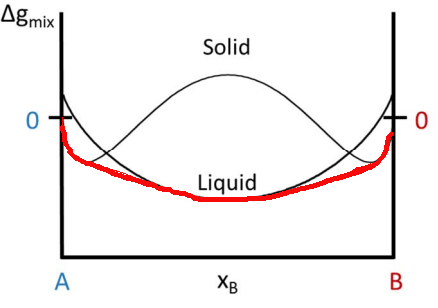
\includegraphics[scale=1]{P3.png}
\end{figure}
\end{document}